%This chapter provides sufficient detail for other scientists to reproduce the experiments presented in the paper. In some journals, this information is placed in an appendix, because it is not what most readers want to know first.





% TODO define a notation for the vIO and the trunk version of the cube re-mapper





\chapter{Materials and Methods}\label{chapter:materialAndMethod}
	The \emph{\notationaio}\space write is a process that allows to limit processor stall during the \emph{\notationIO}\space writing time.   It makes use of independent threads in charge of the effective \emph{write} in memory.   It also requires the usage of different kernel mechanisms (such as interprocess signalling and synchronization) and low-level interfaces (such as \emph{RAM} controller).   A clear vision of the \notationaio\space implementation is mandatory to avoid a dramatic performances collapse while using it.\\

	This chapter first describes the key concepts of our \notationaio\space \emph{write} strategy.   We present the hardware and software requirements of this implementation and the way we have chosen to embed it within the developed applications.\\
	Second, we give a bird-eye view of our two implementations which are based on this \notationaio\space \emph{write} strategy.   The first implementation, which we call the \toolSimulationSoftware\space, is a simplified implementation of the \toolTargetSoftware\space under different \emph{write} strategies (on demand).   The second implementation, which is our main proposal, is a full-fledged version representing our customized implementation of the \toolTargetSoftware.\\
	Furthermore, we present different models for the response time of our proposal.   We use these models to highlight the parameters that influence most the gain of our solutions.\\
	Finally, we describe the experimental set-up and the protocol applied for all our experimental assessments.


%--------------------------------------------
\section{Custom POSIX-based \notationaio\space implementation}\label{section:customAioImplementation}
	\subsection{The POSIX \notationaio\space standard} \label{subsection:AIO_posix_standard}
		The POSIX \notationaio\space (\notationaioShort) standard\cite{bhattacharya2003asynchronous} is a description of an asynchronous access to the \notationIO\space resource.   It is provided by all the Linux operating systems since the Linux 1.3 kernel as the standard "aio" (or "pt\_aio") library.   This UNIX standard library is the angular-stone of all the implementations developed in our work.\\

		Different approaches maybe used to implement an asynchronous access to the \notationIO\space resource.   The one implemented in the POSIX \notationaioShort\space library is based on a work-flow split (see Figure \ref{fig:posixAIO_basis}): when a thread requires an access to the \notationIO\space resource, it simply forwards the request and returns before the request is physically processed.   A dedicated thread (\notationaioWriteThread) is woken up in order to process the effective \notationIO\space access in parallel of the user thread.   The delegated \emph{write} thread becomes in charge of triggering the system call\footnote{Kernel interface to access the \notationIO\space resource} and waiting for the operation to be effectively processed by the kernel.    Then, it may, on demand, alert the initial user thread about the end of the operation.\\
			\begin{figure*}[!h]
				\centering
				\begin{subfigure}[b]{0.7\textwidth}
					\centering
					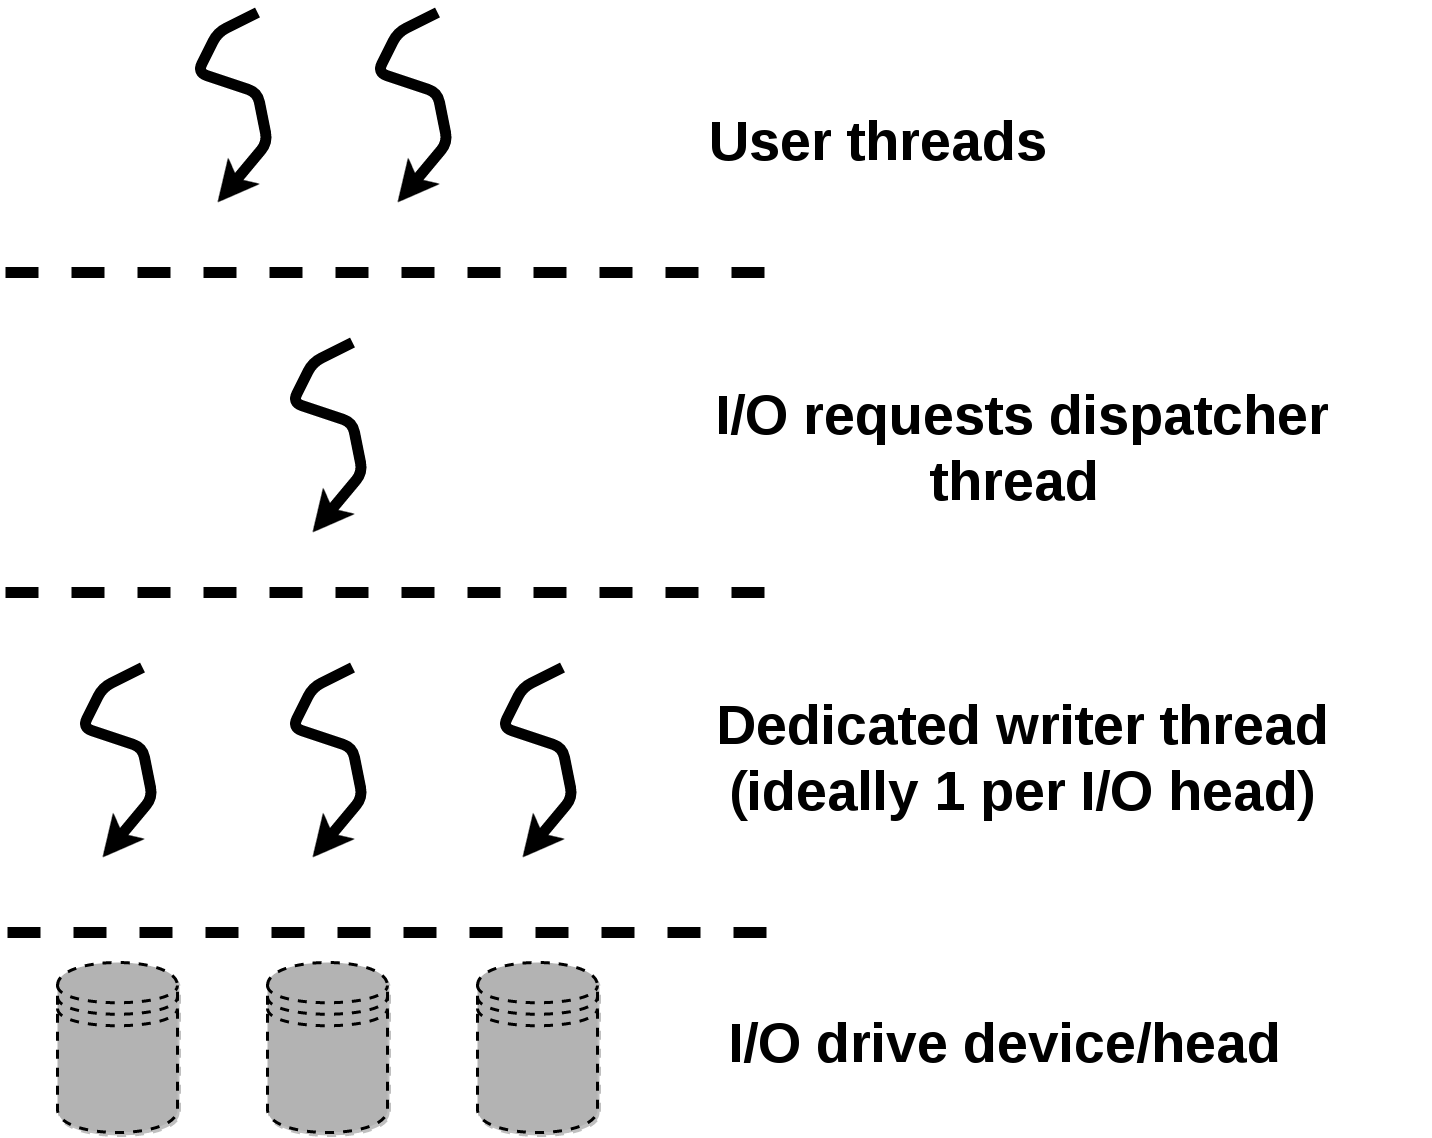
\includegraphics[width=\textwidth]{charts/internship_juelich_posixAIO_basis.png}
				\end{subfigure}
				\caption{POSIX \notationaio\space (\notationaioShort) standard}
				\label{fig:posixAIO_basis}
			\end{figure*}

		Such an approach presents an obvious performance advantage.   The caller thread does not need to wait for the end of the \notationaio\space access.  It might execute other tasks that do not require the end of the resource access.   Given the relatively long time to access the \notationIO\space resource (at processor scale), this might induce a significant reduction of the processor stall time.\\

		Despite these advantages, an intensive usage of the \notationaioShort\space library might be counter-productive in many ways.
		%****** too many writes in parallel *******
		On one hand, the memory footprint of the system may easily sky-rocket, leading to a harmful intensive kernel-swap process (for both user and \notationaioShort\space library threads).   Indeed, each \notationIO\space request may create a potentially large buffer\footnote{The considered buffers are intended to store a memory block which size might be comparable to the live memory (RAM) size.   Hence the explosion of the live memory footprint} which cannot be freed straightforwardly\footnote{In order to allow the user thread to access it asynchronously}.   Given the very small time needed to enqueue an \notationIO\space request, compared to the time to execute it, the user might enqueue a significantly large number of these pending requests.\\

		%******** More threads than IO devices *******
		On the other hand, a miss-calibration of the \notationaioShort\space library\footnote{A calibration that does not suit to the hardware specification.} might lead to a concurrent access to a single \notationIO\space device head, resulting in a dramatic increase of the access time to a given \notationIO\space block.   For instance, let us consider the case where two threads are simultaneously accessing two different blocks\footnote{An \notationIO block is potentially spanning different \notationIO\space sectors} on the same \notationIO\space device (consisting of a single read/write head).   While the head will be scanning a given block, it will be regularly interrupted by requests to scan parts of the other block\footnote{Indeed, scanning a memory block at hardware level is not atomic.   It might have different granularities down to a sector}.   According to Patterson \textit{et al}\cite{patterson1994exposing}, the resulting back-and-forth movement of the \notationIO\space head leads to multiply the access time to a block by up to $10$-fold.\\
		To avoid this hardware interference, all the implementations we present have been tuned to the optimal number of \notationaioWriteThreads: one \notationaioWriteThread\space per \notationIO\space device head.\\

		Our choice of the POSIX \notationaioShort\space library as a foundation of our implementations first aims to limit the engineering effort.   As a matter of fact, the \notationaioShort\space library manages the whole life cycle of all the \notationaioWriteThreads.   It also implements the dispatcher (proxy) thread that receives \notationIO\space requests and forwards them to the \notationaioWriteThreads.   Likewise, the POSIX \notationaioShort\space library might be tuned (number of \notationIO\space devices, number of threads, signal to notify the end of a request process) in order to fit the hardware specifications and the specific \notationIO\space access pattern of the application.\\
		Moreover, the \notationaioShort\space library fits our performance objectives.   Indeed, it efficiently manages, at kernel level, the synchronization of the \notationIO\space resource between the \notationaioWriteThreads.\\
		Considering these services proposed by the \notationaioShort\space library, our engineering effort will focus on the synchronization between the user (caller) thread and the \notationIO\space device-local (\emph{write}) threads.


	\subsection{Synchronizing the \notationaioComputeThread\space and the \notationaioWriteThreads} \label{subsection:synchronization}
		The \notationaioShort\space library manages intrinsically the synchronization between the internal threads that it creates\footnote{Dispatcher and \notationaioWriteThreads}.   It also implements a basic communication mechanism to notify the user about the end of a request's processing\footnote{Effective access to the \notationIO\space resource}.   However, using this mechanism as provided might significantly downgrade the efficiency of the asynchronous strategy within the considered \notationIO\space pattern (see pattern definition in Section \ref{subsection:remapperPattern}).\\
		In this section, we first describe the need we have to implement a synchronization between the user and the \notationaioWriteThreads.   Then, we give an overview of the synchronization mechanism provided by the \notationaioShort\space library.   We explain how it might harm our pattern performances and we describe our solution to enhance it.   Finally, we list the principles that we have followed in our implementations\footnote{Namely the \toolSimulationSoftware\space and the \toolTargetSoftware} to ease and fit this synchronization.\\

		\subsubsection{The need of synchronization}
			%****************** Why we need synchronization (the memory footprint)?
			The main reason why an efficient synchronization mechanism is vital for \notationaio\space is to prevent from memory foot-print explosion.   Indeed, as introduced in Section \ref{subsection:AIO_posix_standard}, the \notationaio\space (and the overlapped accesses to \notationIO\space in general) might lead to a significantly large number of pending requests and of corresponding buffers.   Given the potentially large amount of data carried by these buffers (relative to \notationIO\space disk size), this may easily lead to run out of usable live-memory addresses.   It might also dramatically reduce the overall performances due to the subsequent OS-swap (RAM swap).\\
			By synchronizing the \notationaioComputeThread\space (one that produces the buffers) with the \notationaioWriteThreads\space (those that consume them), the user can expect to access the buffers right after they are processed then remove them.   Hence the reduction of the memory footprint.   However, the important question that remains is: how to make such a synchronization harmless to the performances of the \notationaioComputeThread.   Moreover, how to extend this synchronization in order to regulate the amount of simultaneous buffers before they are created\footnote{This regulation must be triggered on demand: when the memory footprint exceeds a given critical threshold, any creation request should be delayed}.\\

			%****************** Define the AIO synchronization mechanism and its drawback.
			The synchronization mechanism proposed by the \notationaioShort\space library consists in sending a signal (UNIX-kernel signal) to the caller thread after the \notationIO\space request has been effectively processed.   The user thread may decide to execute a custom routine handler to this signal or ignore it.   This mechanism fulfils the synchronization purpose described.   However, two main issues might follow on from its usage.


		\subsubsection{Thread-safety issue of the AIO synchronization}
			The signal handler may compromise the correctness of a critical section between the caller and the \notationaioWriteThreads.   As this signal is received asynchronously, the user (caller thread) cannot decide at which moment to execute the handler.   The handler might thus occur while the caller thread is trying to enqueue a new request to the structure shared with the \notationaioWriteThreads.   As the handler might also require an access to this structure, the single-access principle of this critical section is violated.\\

			%****************** Describe our patch of the nasic AIO synchronization mechanism
			Our solution to avoid thread-safety corruption on the \emph{caller} thread is to forward the execution of the handler to a delegated thread.   This prevents the \emph{caller} execution from being interrupted by any handler.   It also spares the user from implementing a specific critical section to prevent from the handler's execution at inappropriate moments.   


		\subsubsection{Time overhead on the \notationaioComputeThread}
			Executing the handler corresponding to the \notationaio\space signal might create a significant time overhead on the caller (\emph{compute}) thread.   As a mater of fact, this handler interrupts the execution of the caller thread in order to process its own code.   Even more damaging, this handler might require a significant time to process.   It might, for instance, require to access its corresponding buffer\footnote{Buffer which execution has triggered the current handler} (in order to remove it or to check the correct execution of the \notationaio\space request).   Given that this buffer has been processed by another thread (\notationaioWriteThread), its access requires to import it from a potentially distant cache on a potentially distant \emph{NUMA} socket and invalidate it.   Considering the size of such a buffer, this remote \emph{NUMA} node importation is very likely to create false-sharing (see Section \ref{subsection:lightenFalseSharing}).   Hence, the increase of the response time of both the current thread (\emph{caller}) and the one running on the remote \emph{NUMA} node (\emph{writer}).\\

			%****************** Describe our patch of the nasic AIO synchronization mechanism
			Our solution to avoid time overhead on the \emph{caller} thread is the same as that addresses the thread-safety issue.   It consists in forwarding the execution of the handler to a delegated thread.   This allows the \emph{caller} thread to have no delay due to the handler\footnote{Assuming a sufficient number of CPU-cores}.   It also spares the user from implementing a specific critical section to prevent from the handler's execution at inappropriate moments.   Ideally, this delegated thread would be the \notationaioWriteThread\space that has just processed the corresponding request (for core and cache proximity reasons).


		\subsubsection{Improving the \notationaioShort\space synchronization}\label{subsubsection:pthreadWrapper}
			In our implementations, applying any modification to the thread creation and management is not straightforward.   Indeed, these threads are created by the POSIX \notationaio\space library; a UNIX standard library with no certified open-source version available.   Thus, it was not possible to change the thread creation part of this library nor to re-assign the workload between threads.\\
			Our solution was then to wrap up the so-called \emph{pthread} library.\\

			Our solution is to make the thread-creation-request (and few other thread-management-requests) called by the standard \notationaio\space library to be forwarded to our custom wrapper of the \emph{pthread} library.   Our wrapper manages the thread creation and affinity with unique CPU-cores\footnote{The specification and the deployment process of the custom thread library have been released in \href{https://github.com/simbadSid/cubeRemapper\_perfBenchmark}{https://github.com/simbadSid/cubeRemapper\_perfBenchmark}}.   It also allows to attribute custom functionalities to some specific threads.\\

			This solution has led us to build a custom implementation of the \toolTargetSoftware\space referred to as the \emph{\notationaio-pinned thread} version.\\

			Despite the interest of this custom wrapper library, this solution has not been shipped to our final version of the \toolTargetSoftware.   Indeed, wrapping the standard \emph{pthread} library with our custom one requires a non-negligible human intervention before running the \toolTargetSoftware\footnote{For instance, the user would need to set the \emph{LD\_PRELOAD} environment variable with our custom library.   And an unexpected exit of our software would make our custom library be called by default by any other application}.   Such a requirement would make the \toolTargetSoftware\space less user-friendly.   Therefore, unless otherwise specified, our custom wrapper library will not be used in the experiments which will be presented in the next chapter.


	\subsection{Data distribution among threads}\label{subsection:dataDistribution}
		\subsubsection{Custom shared data structure}\label{subsubsection:customDatastructure}
			%****************** Reduced number of shared data and instructions between threads (separated buffer not reused by compute + synchronized queue that allows an optimized access to the only shared structure)
			The two previous solutions aim to enhance the synchronization between the \notationaioComputeThread\space and the \notationaioWriteThread.   The efficiency of such solutions relies on an adequate thread-proximity of the data.   The pattern that we consider is, by design, adapted to such a data distribution (see section \ref{subsection:remapperPattern}).   Our engineering effort has thus focused on the data structure used for the synchronization of the \notationaio\space requests (see Figure \ref{fig:synchronization}).   Our structure implements all the used blocking operations through the \emph{enqueue} and \emph{dequeue} operations.   It also enhances thread proximity by using separate ends for the \emph{enqueue} (\notationaioComputeThread) and \emph{dequeue} (\emph{write} or \emph{handler} thread).\\

				\begin{figure*}[!h]
					\centering
					\begin{subfigure}[b]{0.65\textwidth}
						\centering
						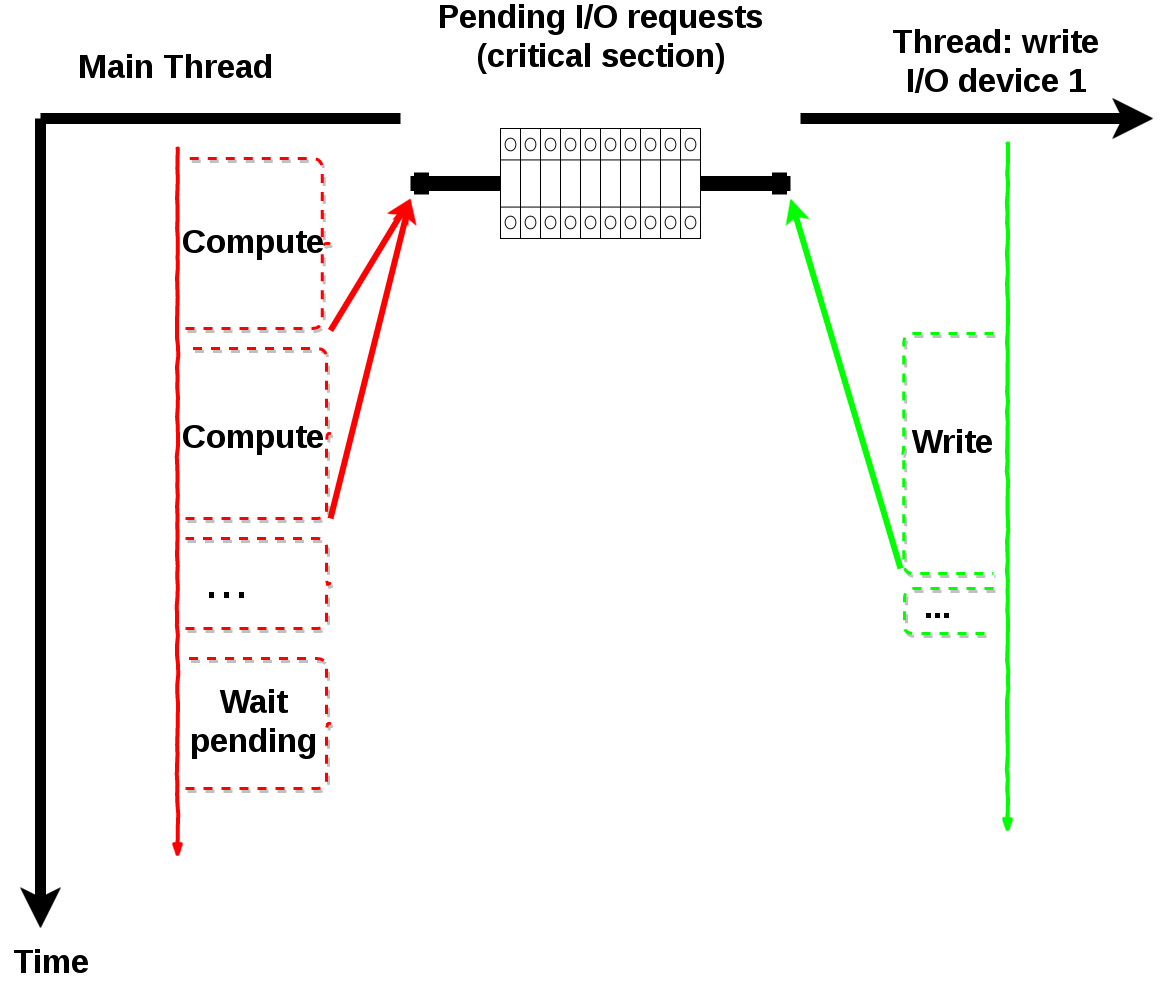
\includegraphics[width=\textwidth]{charts/internshipJulich_AIO-synchronization.png}
					\end{subfigure}
					\caption{Synchronization scheme of the \notationaioComputeThread\space with the \notationaioShort\space threads}
					\label{fig:synchronization}
				\end{figure*}

		\subsubsection{Reducing the impact of \emph{false-sharing}}\label{subsubsection:lightenFalseSharing_concept}
			Among the factors that can limit the efficiency of concurrent algorithms, the shared memory is probably the one that has the deepest impact.   In section \ref{subsubsection:synchronization} we have presented our try to reduce the number of shared memory addresses (at RAM level) and lighten the impact of synchronization between threads.   Let us now reduce even more this shared data impact at cache level.   Our purpose is to address the well-known issue of \emph{false-sharing}.\\

			Let us consider two independent memory buffers used by two concurrent threads.   For clarity, let us also consider that each thread is running on an independent core.   Although the two buffers share no common address, they might still be stored by the same cache line (see Figure \ref{fig:falseSharing_concecpt}).   As the granularity of a cache is a line, then modifying one buffer will lead to the invalidation of the other one.   Likewise, accessing the unmodified buffer will require to import the content of the remote cache line.   Thus a significant overhead at each \emph{read} and \emph{write} access.   This drawback of multithreaded applications is known as \textbf{\textit{false-sharing}}.\\
			Knowing that in our implementation all the concurrent threads (\emph{compute} and \emph{write} operations) are processing \emph{write} accesses, we can easily imagine the high frequency of this costly and idle back-and-forth cache routine.   An assessment of this cost will presented in next chapter (Section \ref{subsection:lightenFalseSharing}).\\

				\begin{figure*}[!h]
					\centering
					\begin{subfigure}[b]{0.55\textwidth}
						\centering
						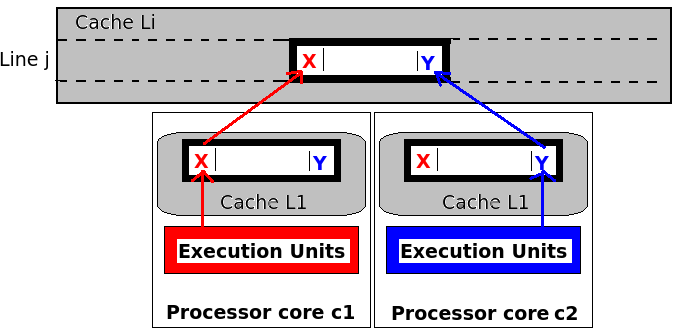
\includegraphics[width=\textwidth]{charts/falseSharing_concecpt.png}
					\end{subfigure}
					\caption{\emph{False-sharing} concept}
					\label{fig:falseSharing_concecpt}
				\end{figure*}

			Our solution to avoid \emph{false-sharing} between concurrent threads is to align each buffer accessed by the concurrent threads to a cache line.   By doing so, we ensure that each buffer is stored within an independent cache line.   Thus, each access to this buffer will be done independently from any other thread.\\

			This solution has led us to build a custom implementation of the \toolTargetSoftware\space referred to as the \emph{\notationaio-buffer aligned} version.

%			Tackling the impact of \emph{false-sharing} on our version of the \toolTargetSoftware\space lead us to a custom implementation referred to as \emph{\notationaio-buffer aligned}.   An evaluation of this version and its improvement is proposed in the next chapter (see Section \ref{subsection:lightenFalseSharing}).

		\subsubsection{Custom dynamic memory allocation}\label{subsubsection:customDynamicMemoryAllocation_concept}
			Let us now see how to go further in limiting the contention on shared data at cache level (primarily L3).   Our objective is to smooth the interaction between the \emph{compute} and the \notationaioWriteThreads.\\
			Our main purpose here is to tackle the dynamic-memory-allocation drawback.   The objective being to make the dynamic memory allocation (invoked at each \emph{compute} operation) less time-consuming and better fit the specification of the allocation-pattern of our application.\\
			To do so, we describe in this section two solutions to undermine the impact of two main performance bottlenecks (relative to multithreading) of a general-purpose memory allocators\footnote{Such as the Linux-standard glibC library: ptmalloc\cite{robertson2003run}}.   Applying this approach on the \toolTargetSoftware\space has led us to implement a custom dynamic memory allocator.\\

			We should mention that our memory allocator has, by design, a significant advantage on the general-purpose allocators (in addition to the three key points described bellow).   Indeed, our allocator is based on a user-level-managed heap chunk.   Thus, the \emph{allocation} and \emph{free} operations require no system calls (unlike the general-purpose allocators).   The inherent advantage of this design choice is not discussed neither assessed in this report.\\

			%***************Take advantage of the specificity of our memory allocation pattern: addresses aligned to ...   Thus we can manage the dynamic memory as a bunch of fixed-size blocks.   Hence no external nor internal fragmentation of the free memory\\
			The first design of our custom memory allocator is to take advantage of the specificity of our memory allocation pattern.   This is done through managing the free memory as fixed-size blocks (unique size equal to a cache line).   Indeed, each allocation needs to be aligned to a given address (see Section \ref{subsubsection:lightenFalseSharing_concept}).  Thus, it is useless to split such a memory block during the allocation: the extra memory (till the next alignment address) will never be required.\\
			Consequently, our dynamic memory management is simplified and reduced to pointer arithmetic.   This considerably reduces the management time and memory footprint.\\
			Our custom allocator has no external fragmentation to deal with.   Meanwhile, the effect of the created internal fragmentation is lightened by the OS: as the extra addresses are not know by the user, they will most likely never be used.   Thus, the OS will swap them out\footnote{As a memory blocks has a cache-line size, it will be swapped out into single page.   It will also create no residual in the RAM}, which will almost completely remove any time and memory space impact.\\

	%		***************Improve the synchronization between allocation (compute) and free (write) which might be made by independent threads\\
			The second design we came with is to store our free memory blocks within a structure with two independent ends:  one to allocate a block and the other to return a freed block (see Figure \ref{fig:customMemAlloc_freePool}).   Indeed, when couple with our \notationaio\space strategy, this structure ensures that the thread that allocates memory (the compute thread) is not the one that frees it (after the write thread work).   Thus, our distributed architecture allows to soften the contention on the shared free memory structure.  As the \emph{free} operation may be processed in parallel, we have designed the \emph{free} end of the shared memory structure as a "Treiber" stack \cite{pedersen1998method}:   a lock free stack that ensures thread-safety using the hardware atomic primitive: \emph{compare-and-swap}\cite{valois1995lock}.   This ensures a thread-safety to this structure without any software synchronization.\\
				\begin{figure*}[!h]
					\centering
					\begin{subfigure}[b]{0.7\textwidth}
						\centering
						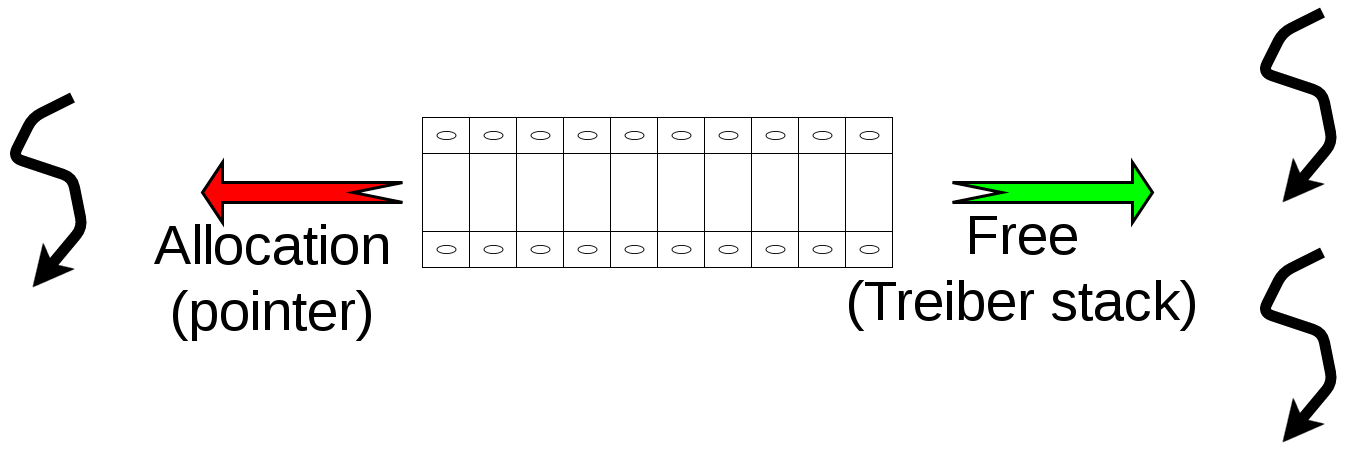
\includegraphics[width=\textwidth]{charts/internship_juelich_customMemAlloc_freePool.png}
					\end{subfigure}
					\caption{Free dynamic memory architecture}
					\label{fig:customMemAlloc_freePool}
				\end{figure*}

			The incorporation of this custom memory allocator has led us to build a custom implementation of the \toolTargetSoftware\space referred to as the \emph{\notationaio-full-fledged} version.


	\subsection{The \toolTargetSoftware\space custom implementation (asynchronous)} \label{subsection:remapperPattern}
		%****************** The main objective of the whole work: optimize the response time of this software
		As described in Section \ref{section:cubeRemapper_stateOfTheArt}, the execution time of the \toolTargetSoftware\space has a significant portion of processor idle time.   Indeed, at each iteration of this software, the \emph{compute} operation is followed by a \emph{write} operation.   Due to the important amount of data stored on the hard disk, this operation has a significant impact on the overall execution time.\\
		Our objective is to reduce the stall time of the processor by overlapping the \emph{compute} with the cause of the processor stall: the \notationIO\space \emph{write} function.   The \notationaioShort\space library and the custom synchronization method that we have previously described are the foundations of the improvement we want to bring to the \toolTargetSoftware.\\

		\begin{figure*}[!h]
				\centering
				\begin{subfigure}[b]{0.33\textwidth}
					\centering
					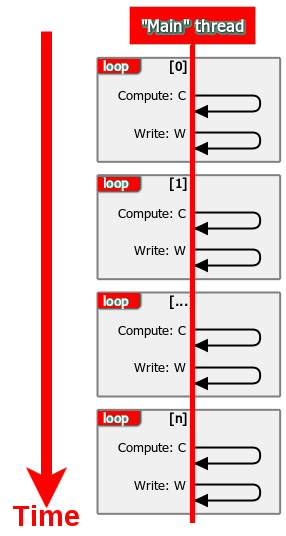
\includegraphics[width=\textwidth]{charts/internshipJulich_model_0-IO-simple.png}
					\caption[Synchronous case]
					{{\small Synchronous case}}
				\end{subfigure}
				\hfill
				\begin{subfigure}[b]{0.475\textwidth}  
					\centering
					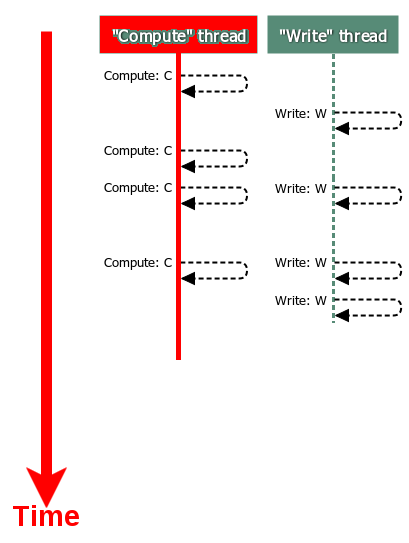
\includegraphics[width=\textwidth]{charts/internshipJulich_model_0-AIO-simple.png}
					\caption[]%
					{{\small Asynchronous case}}
				\end{subfigure}
				\caption{\notationAIO\space applied to the \toolTargetSoftware\space pattern}
				\label{fig:AIO_basis}
			\end{figure*}

		%****************** Describe the simulation test-bed implementation
		The main idea behind our implementation of the \toolTargetSoftware\space is summarized in Figure \ref{fig:AIO_basis}.   Let us consider the main loop of the \toolTargetSoftware.   Thanks to the \notationaioShort\space library, we expect to overlap the execution of each \emph{write} operation with one of the next computations.\\
		For such a strategy to succeed, one must ensure that the two operations (\emph{compute} and \emph{write}) are using totally independent memory addresses (except the one used for the synchronization).

	\subsection{The \toolSimulationSoftware} \label{subsection:simulationTestbed}
		In order to assess the solution we propose for the \toolTargetSoftware, one could simply ship it to the \toolTargetSoftware\space and evaluate its performances.   However, the \emph{compute} operation of the \toolTargetSoftware\space involves different and highly-random memory access patterns (at RAM level).   It also allocates and deals with significantly large chunks of the process stack.   Thus, it might have unexpected impacts on the \emph{write} operation that we implement.   It might also have a performance impact on the synchronization between the \notationaioComputeThread\space and the \notationaioWriteThreads.   Finally, it might be extremely sensitive to remote memory-accesses on the data it generates\footnote{The interferences (between concurrent threads) that we consider here take place mainly at cache level.   At RAM level, such an interaction is harmless due to the synchronization we have designed}.   In Section \ref{section:experimentalCase}, we will present an experimental assessment of this potential interferences and we will show the huge impact that they might have on our implementation of the \toolTargetSoftware\space (basic version).\\

		To avoid dealing with these interferences (in a preamble step), we have decided to simplify the global pattern of the \toolTargetSoftware\space through a custom and independent program (\toolSimulationSoftware).   This \toolSimulationSoftware\space allows to reduce the response time of the system down to the two operations: \emph{compute} and \emph{write}.   It also gets ride of the numerous potential sources of perturbation by simplifying these two operations.   It is used as a preliminary test for our theoretical models.\\
		At the same time, our simulator may use different strategies to simulate the complex \emph{compute} operation of the \toolTargetSoftware.   This allows to observe different behaviours of the \toolTargetSoftware\space without having to find the inputs that would trigger such a behaviour.   One may, for instance, observe different \emph{compute} times or live-memory access patterns.   From a purely theoretical perspective, our \toolSimulationSoftware\space allows to assess different aspects of the \toolTargetSoftware\space pattern within different domains.   This intends to confirm the potential performance gain of our solution.   It would also help us identify the domain where such a gain would be optimal.\\

		The main principle behind the \toolSimulationSoftware\space is described on the listing \ref{code:simulator}.   The algorithm used for the \emph{compute} and the \emph{write} operations are set through the usage of different implementations of the same "Worker" interface.\\
		\begin{minipage}{\linewidth}
			\begin{lstlisting}[language=C++, caption={\toolTargetSoftware\space \toolSimulationSoftware}, label={code:simulator}]
int main(int argc, char **argv)
{
    unsigned int nbIteration, computeTime, bufferSize, nbIoDevice, nbProc;

    extractParameter(argc, argv, &nbIteration,
                     &computeTime, &bufferSize, &nbIoDevice,
                     &nbProc, &memAccessPattern);
    // Pick the implementation to use for the "compute"
    // and the "write" operations
    Worker worker = Worker.generate(nbIteration, computeTime, bufferSize,
                                    nbIoDevice, nbProc);

    for (int i=0; i<nbiteration; ++i)
    {
        char *buffer = worker.compute();
        worker.write(buffer);
    }

    worker.waitPendingRequest();

    return 0;
}
			\end{lstlisting}
			\end{minipage}
		This code also shows the main parameters of the simulation that might be tuned:
		\begin{itemize}
			\item Number of iterations
			\item Compute time (per iteration)
			\item Number of hardware \notationIO\space devices (used to determine the number of concurrent \notationaioWriteThreads)
			\item Number of concurrent CPU-cores (used to initialize the \notationaioShort\space library internal thread synchronization)
			\item Buffer size used at each computation
		\end{itemize}


%--------------------------------------------
\section{Proposed theoretical models}\label{section:model}
	In this section, we propose two theoretical models for the response-time of our custom (\notationaio) implementations.   We also try to enhance these models in order to fit the HPC platform specifications (multiple parallel \notationIO\space devices and reduced computation time).\\
	These models are used to determine the parameters\footnote{Example: \emph{compute} time, \emph{write} buffer size} that influence most our solution.     They will also help us (in Section \ref{subsection:AIO_firstApproachAssessment}) to confirm the potential gain brought by our solution (from a theoretical perspective).   Finally, they will help us determine the domain where our solution may bring a significant improvement.\\

	Clearly, the gain brought by our proposed algorithm will be compared to the existing synchronous model given by the following Equation (\ref{equation:synchronousModel}):
	\begin{equation}
	\begin{aligned}
		T_{synchronous}	= n * (C + W)
		\label{equation:synchronousModel}
	\end{aligned}
	\end{equation}
	In this model, all the instructions are serialized.   Thus, the total execution time is simply the sum of all the execution times.\\

	To conduct our experimentations, we assume that the size of the buffer written at each iteration is constant (for a given experimentation).   We also assume that the computation time $C$ at each iteration is constant (for a given experimentation).\\
	The following notations are used to express the theoretical model of our asynchronous version of the \toolTargetSoftware:
	\begin{itemize}
		\item $C$: computation time at each iteration
		\item $W$: size of the buffer written at each iteration
		\item $n$: number of iterations
		\item $P$: number of computation-cores available
		\item $N_{io}$: number of independent \notationIO\space access heads (only used in section \ref{subsection:multipleParallelIoDevice})\\
	\end{itemize}


	\subsection{First approach: simple write/compute representation (single \notationIO\space device)} \label{subsection:firstModel}
		In this first approach, we present a simple model by introducing the following hypotheses:
		\begin{itemize}
			\item Constant writing time $W$ of each buffer.
			\item Perfect parallelization model (execution time with $p$ computation cores $T(p) = \frac{T(1)}{p}$).
		\end{itemize}
		Thus, the execution time of the asynchronous pattern would be:
			\begin{equation}
			\begin{aligned}
				T_{asynchronous}&= C + W + (n-1) * max(C , W)
			\end{aligned}
			\label{equation:model0}
			\end{equation}
		Indeed, the first computation time and the last writing time (the two first terms of the above equation) cannot be avoided or softened.   Then, the \emph{compute} and the \emph{write} operations are executed by two independent threads (ideally with no interference between them).   Hence, we only retain the maximum execution time of the two threads: $max((n-1)*C, (n-1)*W) = (n-1) * max(C, W)$.\\

		In this model and for the seek of simplicity, we deliberately get ride of the scheduling and pseudo-parallelization\footnote{Pseudo-parallelization happens when 2 concurrent threads are executed on the same mono-threaded core} overhead.   This decision is also motivated by the limited impact of these phenomena regarding the range of the considered writing and computing times (see the \emph{write} time evaluation in Section \ref{subsection:AIO_firstApproachAssessment}).\\

		By analysing the asymptotic behaviour of Equation (\ref{equation:model0}), one may use the following approximations:
			\begin{equation}
			\begin{aligned}
				T_{asynchronous}	\stackrel{\text{if C << W}}{\approx} n * W + C
									\stackrel{}{\approx} n * W
			\end{aligned}
			\label{equation:model0:C<<W}
			\end{equation}
			\begin{equation}
			\begin{aligned}
				T_{asynchronous}	\stackrel{\text{if C >> W}}{\approx} n * C + W
									\stackrel{}{\approx} n * C
			\end{aligned}
			\label{equation:model0:C>>W}
			\end{equation}


	\subsection{Second approach: modelling the perturbations (single \notationIO\space device)} \label{subsection:secondModel}
		The previously-generated model allows a simple estimation of our version of the \toolTargetSoftware\space pattern.   However, it relies on hypotheses that make it hardly scalable.
		While trying to enhance this model, we have experimentally observed (see Section \ref{subsection:AIO_firstApproachAssessment}) that the difference between the theoretical model and its experimental evaluations seems constant (with respect to the computation time).   Based on this finding, we propose the following improved second model:
			\begin{equation}
			\begin{aligned}
				T_{asynchronous}&= C + W_{perturbation} + (n-1) * max(C , W_{perturbation}) + n * req
			\end{aligned}
			\label{equation:model1}
			\end{equation}
		Where:
		\begin{itemize}
			\item $req$ is the time to transmit the \emph{write} request (or enqueue it for later execution).
			\item $W_{perturbation}$ is the delay of the \emph{write} operation introduced by the payload and the contention on the \notationIO\space device.
		\end{itemize}
		In this second model, we try to express the previously-observed perturbations\footnote{Gap between the theoretical model and the experimental evaluation} by introducing the two expressions $req$ and $W_{perturbation}$.   These two expressions do not depend on the computation time; hence, each one of them can potentially explain the constancy of the observed perturbation.\\

		\subsubsection{Modelling the writing time ($W_{perturbation}$)}\label{subsubsection:modelWritingTime}
			% Context
			When we estimate the overall time response of the \toolTargetSoftware\space pattern, the experimental errors of the \emph{write} time at each iteration are summed up.   This may eventually have a significant impact on the total response time.  In this section, we no longer consider the \emph{write} time as constant and try to fit more accurately its variations.\\

			% Identify the pb: write time is not constant
			Providing an accurate measurement of the \emph{write} time maybe very complex (even when we consider buffers with constant sizes).   The \emph{write} time may highly vary depending on the processor family\footnote{Here we mainly refer to the number of cores and physical threads.}, the previously processed \notationIO\space requests, the detected \notationIO\space access pattern\cite{petrovic2015performance}, or even some unexpected external parameters (such as the system temperature or some magnetic interferences)\cite{lu2003performance}.
			% Reason why we initially did this hypothesis
			However, we still need to estimate it to validate our theoretical model.\\
			% Our solution

			Our solution to overcome this difficulty is to consider the writing time as constant but only at saturation regime.   This solution is inspired from the "I/O saturation method" introduced by R. Robert \emph{et al}\cite{ross2001case}.   It consists in measuring the time to write a given buffer after flooding the \notationIO\space system with concurrent \emph{write} access (following a given access pattern).   In order to measure the required \notationIO-saturation level\footnote{Depends on the hardware \notationIO\space specification} and apply the \notationIO-saturation during the write-time measurement, we have used the code released by the above-cited reference.\\

		\subsubsection{Modelling the \notationaio\space request time ($req$)}\label{subsubsection:modelRequestTime}
			Let us consider an \notationaio\space request submitted by the \emph{compute} thread.   Such requests are always processed by the main thread in the considered approach.   Thus, their time foot-print cannot be avoided neither divided upon processor cores or \notationIO\space devices.\\
			Within the scope of our study, we consider the \notationaio\space request-time as constant (for a given hardware platform).   Indeed, submitting an \notationaio\space corresponds to simply forward the request-address from the \emph{compute} thread to the \emph{write} thread.   No other computation nor data transfer is performed at this step\footnote{The buffer to be written might be imported by the writer thread later-on when the effective \notationIO\space operation will be processed}.\\

			Our method to evaluate the \notationaio\space request-time\footnote{For a given hardware platforms} is similar to the \notationIO\space write-time evaluation (see Section \ref{subsubsection:modelWritingTime}).   It consists in assessing the time $T$ to submit an \notationaio\space request for different number $n$ of iterations (number of requests submitted): $T = req * n$.   Then, determining $req$ is equivalent to determining the linear model that fits the best the assessed values $(T, req)$.\\

			Thanks to the generated linear-model, we can determine the value of the request time as the slope of the linear model.   We may also confirm our hypothesis (constant \notationaio\space request-time) using the constant term\footnote{Other methods could be applied in order to assess the validity of the linear model (example: the "coefficient of determination" $R^{2}$).   But these would require a benchmark evaluation of the acceptable error}.\\


	\subsection{Introducing multiple parallel \notationIO\space devices} \label{subsection:multipleParallelIoDevice}
		In this section, we suppose that the hardware platform has at its disposal $N_{io}$ independent \notationIO\space devices.   Hence, at most, $N_{io}$ independent \notationIO\space operations maybe performed concurrently.   For simplicity, we assume in this section that the parallel \notationIO\space model is perfect: two concurrent \notationIO\space operations on two different \notationIO\space devices will not create any interference on each others.   We also assume that the number $N_{io}$ of \notationIO\space devices is much smaller than the number $n$ of iterations (for the simplicity of the model expression).\\

		Thanks to Equation (\ref{equation:model0:C>>W}), we can notice that when $C >> W$, the time response of our system does not depend on the writing time $W$\footnote{However $W$ appears in this equation, it is a simple added element with no coefficient.   Thus this write time $W$ can not be split over multiple devices.}.   Thus, introducing additional parallel \notationIO\space devices will not affect this response time (see Figure \ref{subFig:model0_multipleIoDevice_C>>W}).   Hence, our model in this case remains:
			\begin{equation}
			\begin{aligned}
				T_{asynchronous}(N_{io})	\stackrel{\text{if C >> W}}{\approx} n * C + W
											\stackrel{}{\approx} n * C
			\end{aligned}
			\end{equation}
		By simply extending this model to the case where $C \approx W$, we can see (Figure \ref{subFig:model0_multipleIoDevice_C=W}) that additional \notationIO\space devices are still useless.   The model in this case remains:\\
			\begin{equation}
			\begin{aligned}
				T_{asynchronous}(N_{io})	\stackrel{\text{if C = W}}{\approx} n * C + W
											\stackrel{}{\approx} n * C
			\end{aligned}
			\end{equation}
			\begin{figure*}[!h]
				\centering
				\begin{subfigure}[b]{0.475\textwidth}
					\centering
					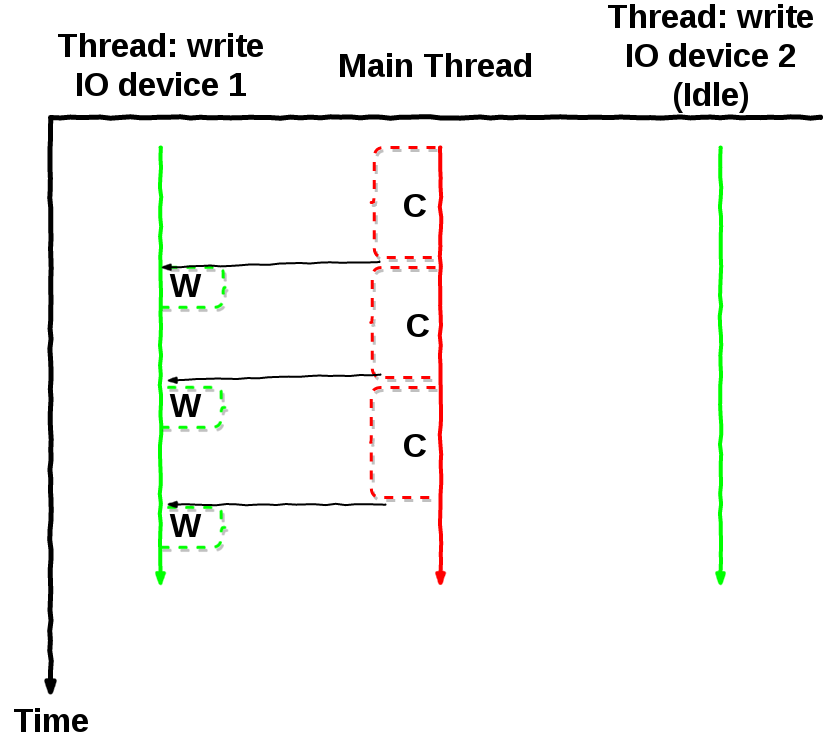
\includegraphics[width=\textwidth]{charts/internshipJulich_AIO-multipleIoDevice_CBiggerThanW.png}
					\caption[Computation time $>>$ Write time]%
					{{\small Computation time $>>$ Write time}}
					\label{subFig:model0_multipleIoDevice_C>>W}
				\end{subfigure}
				\hfill
				\begin{subfigure}[b]{0.475\textwidth}  
					\centering 
					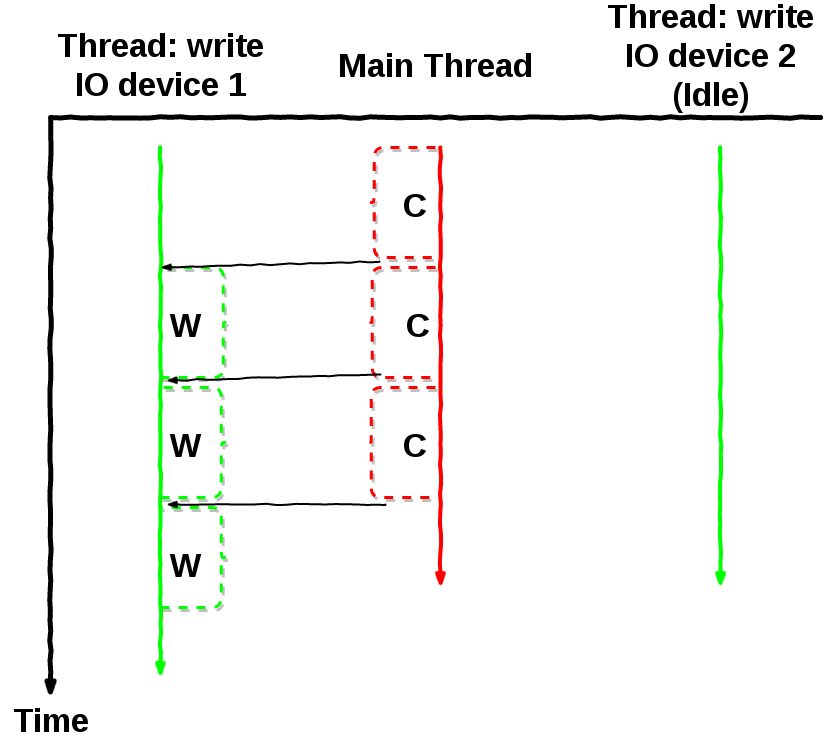
\includegraphics[width=\textwidth]{charts/internshipJulich_AIO-multipleIoDevice_CEquivalentToW.png}
					\caption[]%
					{{Computation time $\approx$ Write time}}
					\label{subFig:model0_multipleIoDevice_C=W}
				\end{subfigure}
				\vskip\baselineskip
				\begin{subfigure}[b]{0.475\textwidth}
					\centering
					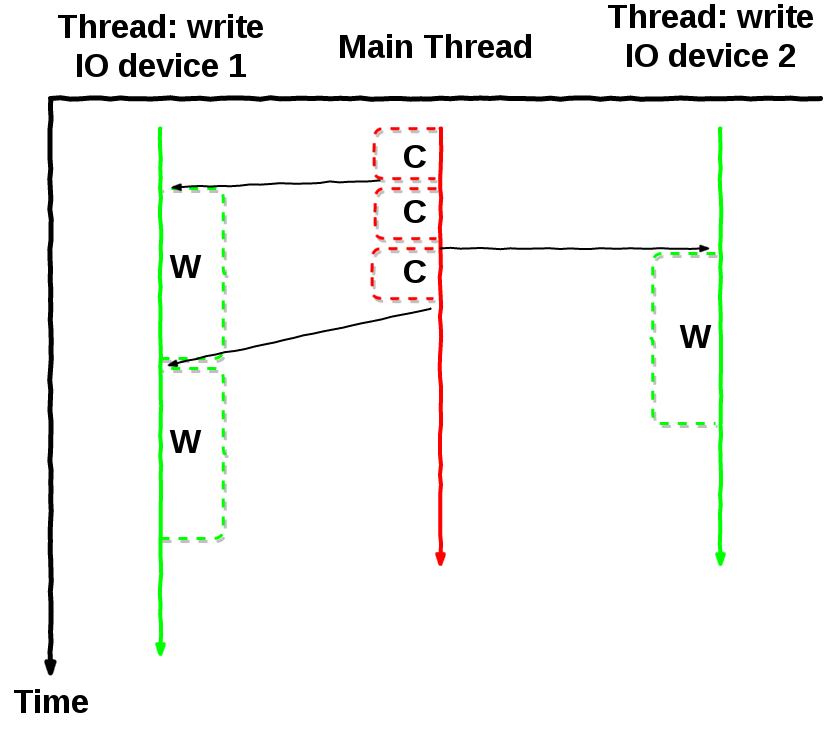
\includegraphics[width=\textwidth]{charts/internshipJulich_AIO-multipleIoDevice_CSmallerThanW.png}
					\caption[]%
					{{\small Computation time $<<$ Write time}}
					\label{subFig:model0_multipleIoDevice_C<<W}
				\end{subfigure}
				\caption[Asynchronous \notationIO\space pattern diagram with multiple \notationIO\space devices]
				{\small Asynchronous \notationIO\space pattern diagram with multiple \notationIO\space devices}
				\label{fig:model0_multipleIoDevice}
			\end{figure*}
		Finally, in the case where $C << W$, the number of \notationIO\space devices becomes relevant (see Figure \ref{subFig:model0_multipleIoDevice_C<<W}).   The new inflection point (computation time where this model becomes applicable) is $C = \frac{W}{i}$.   The theoretical model in this case becomes:\\
			\begin{equation}
			\begin{aligned}
				T_{asynchronous}(N_{io})	& \stackrel{\text{if C << W}}{\approx} (n-1) * max(\frac{W}{N_{io}}, C) + C + W			\\
				T_{asynchronous}(N_{io})	& \stackrel{\text{if C << }\frac{W}{N_{io}} }{\approx} (n-1) * \frac{W}{N_{io}} + C + W		\\
				T_{asynchronous}(N_{io})	& \stackrel{\text{if C } \in [\frac{W}{N_{io}}, W] }{\approx} (n-1) * C + C + W
											\stackrel{}{\approx} n * C + W
			\end{aligned}
			\label{equation:model0_multipleIoDevice_C<<W}
			\end{equation}


%--------------------------------------------
\section{Target hardware platform and compatibility}
	\subsection{Hardware platform}
		%******************  Need to a highly multithreaded (physical thread) machine:
		The performance profiling and measurement tools that we are developing are intrinsically designed for highly-multithreaded (physical thread) hardware platforms.   There principle purpose is to track and profile performance-bottlenecks that are due to the contention of concurrent (threads or processes) execution.   These tools aim to assess each unitary\footnote{Thread, process or job execution} execution.   They also aim to evaluate the communication and the interaction between these executions\footnote{\emph{MPI} or kernel-level (ex: pipe, socket) communication}.   These dimensions can only be set and observed on a hardware platform that physically\footnote{In this study we do not consider virtual hardware environments.} allows an execution at such concurrent scale.\\

		%****************** Why HPC platform?
		As we consider highly-concurrent hardware platforms, HPC platforms are obvious candidates.   For the experimental assessment of our study, we made such a choice (see section \ref{section:experimentalSetup})  for both practical and functional intends.\\

		On one hand, our study has been conducted within an environment of cutting-edge HPC-specific performance track researches.   Our goal to outperform the \toolTargetSoftware \cite{saviankou2015cube} is part of a global project\footnote{Scalasca project\cite{zhukov2013assessing}} that aims to develop a set of tools that provide highly scalable performance measurement and analysis for computation at HPC scale.   Our work is thus part of a framework to enhance and automate the profiling of parallel and distributed applications at HPC scale.\\

		On the other hand, an HPC platform represents an ideal experimental set-up for our theoretical study about overlapped \notationIO-accesses.   The HPC platforms we considered (see Section \ref{section:experimentalSetup}) has at its disposal several parallel and independent \notationIO\space devices, managed by a shared file system.   Moreover, as mentioned in Section \ref{subsection:AIO_posix_standard}, the number of concurrent \notationaioWriteThreads\space is limited by the number of independent \notationIO\space devices.   Hence, thanks to the HPC's numerous independent \notationIO\space devices, one could expect that the \notationaio would bring a significant additional gain.\\

		Thanks to the specification of the considered HPC hardware (see Section \ref{section:experimentalSetup}), the overlapping and the parallelization implemented by our solution maybe reached with a reduced time overhead.   In this context, the high number of CPU-cores and the large cache size are two commonly-considered helping factors.   However, the \emph{Hyper-Threading} technology\cite{magro2002hyper}\footnote{The \emph{Hyper-Threading} technology is not specific to the HPC platforms.   It is an \emph{Intel} technology that is also deployed on some modern Intel servers} is probably the most influencing design of such a hardware architecture on our approach.\\
		The \emph{Hyper-Threading} technology allows two threads to run concurrently on the same CPU-core:   there relative micro-instructions (except the load/store instructions) being processed in parallel as if they where running on two distinct CPU-cores.   As shown in Figure \ref{fig:hyperThreading}, the advantage of such a design, compared to physical parallelization\footnote{Two concurrent threads running on two independent CPU-cores}, comes from the optimal cache proximity of the shared data at all cache levels (L1, L2, L3 (data and instruction) and \emph{Translation Lookaside Buffer}).\\
		In the ideal case, this would allow the \notationaioComputeThread\space (producing the buffers) and the \notationaioWriteThread\space (consuming the same buffers) to run simultaneously on the same CPU-core.   By doing so, we take advantage of the parallelization\footnote{Unlike pseudo parallelization where two concurrent threads run on the \emph{same CPU-core} by interrupting each others}.  Additionally, the shared buffer will not need to be moved from the producer core to the consumer core.   Hence the optimal cache proximity.\\
		The same cache proximity advantage can be noticed on the \emph{Translation Lookaside Buffer} (TLB).   The address translation\footnote{Virtual-physical and physical-virtual address translation} used by the \notationaioComputeThread\space is similar to the one used by the \notationaioWriteThread\space (in the specific execution case described earlier).   Thus, the content of the TLB might be reused by the \notationaioWriteThread\space without cache-misses.\\

			\begin{figure*}[!h]
				\centering
				\begin{subfigure}[b]{0.48\textwidth}
					\centering
					\frame{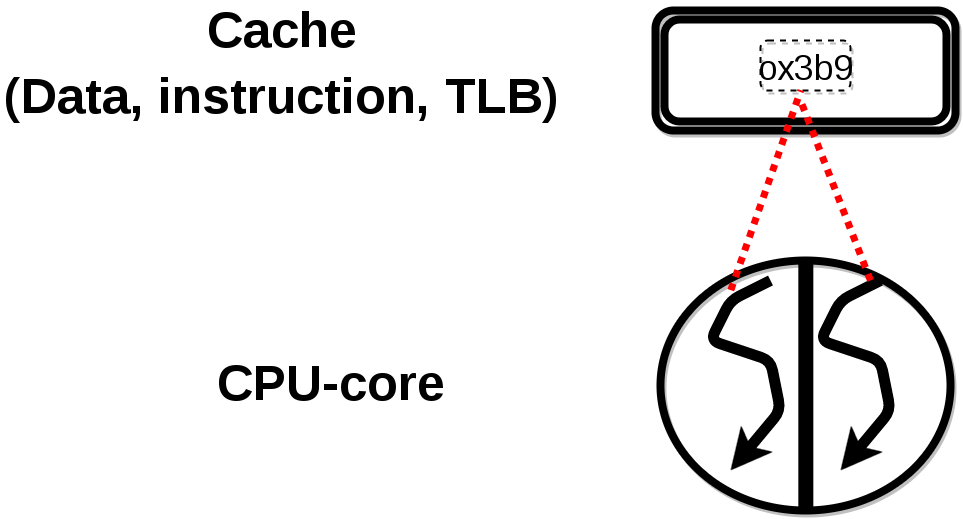
\includegraphics[width=\textwidth]{charts/internshipJulich_hyperthreading.png}}
					\caption[Hyper-Threaded core]
					{{\small Hyper-Threaded core}}
				\end{subfigure}
				\hfill
				\begin{subfigure}[b]{0.48\textwidth}  
					\centering
					\frame{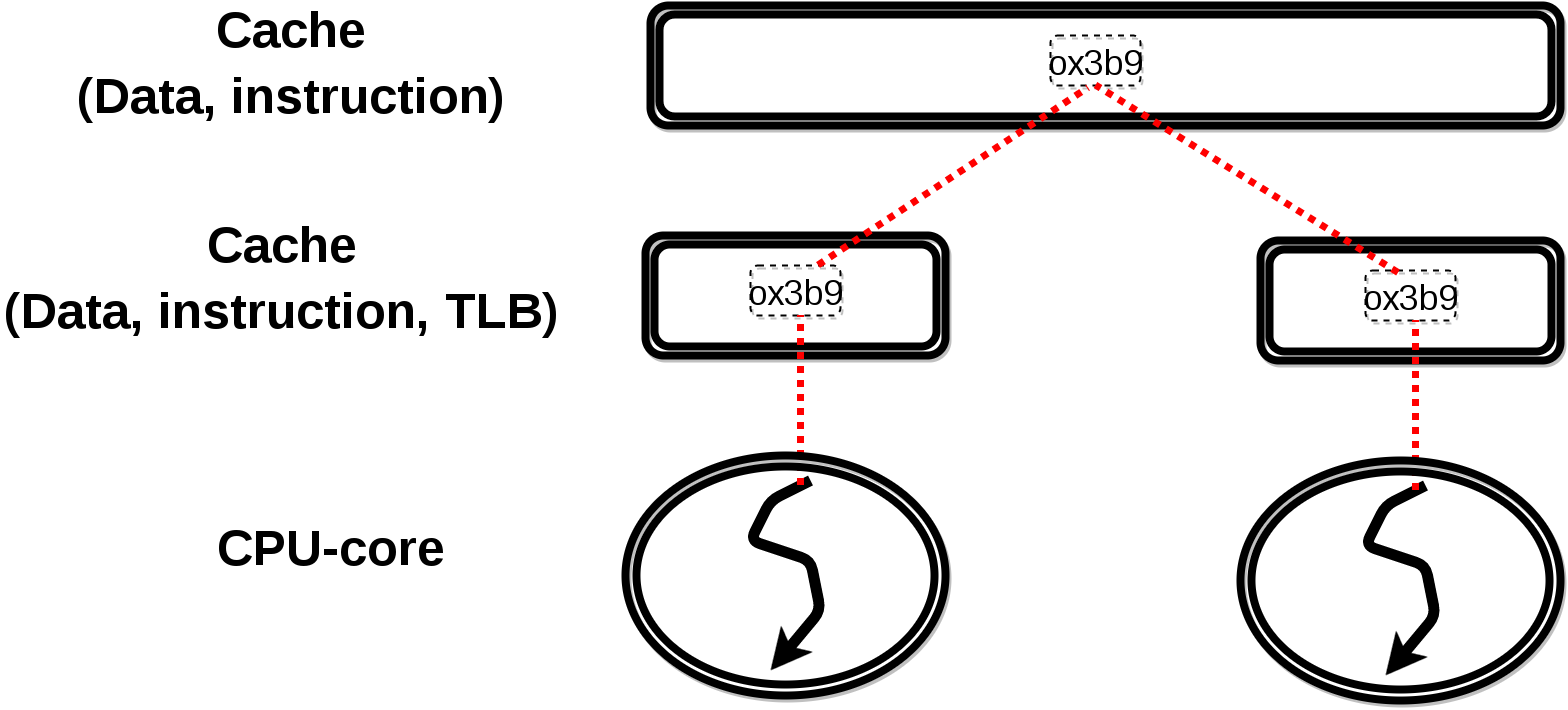
\includegraphics[width=\textwidth]{charts/internshipJulich_multicore.png}}
					\caption[]%
					{{\small Multi-core}}
				\end{subfigure}
				\caption{\emph{Intel}'s Hyper-Threading technology concept}
				\label{fig:hyperThreading}
			\end{figure*}

		It is worthwhile to mention that the thread-distribution advantage brought by the \emph{Hyper-Threading} to our overlapping solution is highly random.   Moreover, it cannot be controlled nor enforced at software (user or kernel) level.   The evaluation of such an impact on our solution is out of the scope of this study.


	\subsection{Operating-system portability} \label{subsection:osPortability}
		The main family of operating-systems (OS) targeted by our research and implementations is the \emph{UNIX}-like system\cite{wikipediaUNIX} (with a primer for \emph{Gnu-Linux} OS).   The reasons for this choice are relative to both implementation-compatibility and kernel-level requirements.\\

		%****************** Most of the HPC ecosystem is UNIX-compatible
		On one hand, our global project (\emph{Scalasca}) aims to develop an HPC utility (\toolTargetSoftware).   As a matter of fact, the HPC ecosystem is well known for its dependency on UNIX-like systems.   To the best of our knowledge, only few alternative systems\footnote{The main example is the \emph{Microsoft Windows} HPC Pack 2008.   But even this project has been dropped by \emph{Microsoft} and is no longer supported} exist for the UNIX-dominated HPC market.   No future evolutions seem likely to affect this trend.   Consequently, deploying our version of the \toolTargetSoftware\space on non \emph{UNIX}-like systems would have no real practical interest.   Such a release would target an insignificant set of potential users.\\

		%****************** Pur implementation uses UNIX-specific mechanisms
		On the other hand, the whole idea beneath our asynchronous approach is based on mechanisms that are generally specific to \emph{UNIX} architectures.   For instance, let us consider the synchronization that we have implemented between the \notationaioComputeThread\space and the \notationaioWriteThreads\space (see Section \ref{subsection:synchronization}).   Our intend was to reduce the memory footprint and ease the communication between the producer and consumers of the \notationIO\space requests.   To do so, we have made use of interprocess signals as well as condition pipes: event-driven communication.   Such a programming paradigm is intrinsically linked to the process-design of \emph{UNIX} platforms;   hence the difficulty to consider this paradigm for non-\emph{UNIX} deployment.\\
		Some state-of-the-art libraries allow to emulate \emph{UNIX}-specific mechanisms on non \emph{UNIX} platforms \cite{robison2012cilk}.   However, such solutions are not natively implemented by these systems\footnote{Unlike the signal and all event-driven mechanisms on \emph{UNIX}-compatible OS (implemented and executed at kernel level)}.   Thus, their usage may lead to a significant time and memory overhead due to extra system-calls and interprocess polling;  not to mention the obvious library- and name-space-compatibility issues.\\

		Despite this compatibility limitation, we still have considered \emph{windows}-OS portability for our implementation of the \toolTargetSoftware.\\
		% ******************Issue on windows
		The main issue when we consider deploying a multithreaded \emph{UNIX}-based application on \emph{windows} comes from the thread-synchronization:   unlike most \emph{UNIX}-based OS architectures, the \emph{windows} OS does not natively implement signals and related event-oriented mechanisms.   Thus, the whole work-flow of our multithreaded algorithm can no longer be implemented.\\
		% ******************Considered solution
		Our solution to deploy the \toolTargetSoftware\space on \emph{windows} platforms was to use the \emph{Cilk Plus}\cite{robison2012cilk} library \footnote{Library proposed by \emph{Intel} to emulate \emph{UNIX} process and relative thread-synchronization mechanisms on \emph{windows} platforms at user level (user mode)}.   Then, through a custom wrapper of this library, we have been able to fit all the kernel-level requirements of our algorithms and benchmarks.   Using this wrapper, we have also limited the engineering effort by adapting this interface to the standards followed by the \toolTargetSoftware\space (name spaces, function names and parameters).\\
		% ******************Potential limitation of the solution
		This kind of user-level emulation of a kernel process is well known for its potential performance downgrade\cite{tousimojarad2014comparison}.   Indeed, the \emph{Cilk Plus} library manages the process address-space (and principally the heap's dynamic memory) through costly system calls to the host kernel (instead of being natively executed by the kernel).   Likewise, the implementation of these signals and these synchronizations is based on \emph{active-waiting} and \emph{polling}.\\
		The assessment of such an overhead on our asynchronous approach (deployed on \emph{windows} OS) is beyond the scope of this work.\\

		For simplicity and clearness, all the considered implementations in the rest of this work will be implicitly developed, implemented and assessed on UNIX platforms.


	\subsection{Experimental setup}\label{section:experimentalSetup}
		% ****************** Hardware platform: HPC (Processor + disk)
		The experimental evaluations that will be presented in the next chapter have been obtained on two x86 machines.\\
		The first one is a \emph{JURECA T-Platforms V-Class} (HPC) consisting of two 24-core (\targetPlatformHpcProcessor\space (\targetPlatformHpcFrequency) \emph{Haswell}) chips.   Each core has a double physical thread support (\emph{Hyper-Threading}).   The machine accesses its \notationIO\space resource using \emph{JUST}\cite{just}: a \emph{General-Parallel-File-System} storage cluster.   Thanks to the hardware distribution of its underlying disks, this file system may perform (\emph{physically}) several simultaneous accesses to the \notationIO\space resource.   The access to this file system is performed through a $100$ GiB/s connection.   Finally, on this machine, a \emph{Gnu-Linux} (3.10.0-514.26.2.el7) operating system has been used based on the \emph{CentOS} kernel (7.3.1611).   The default kernel dynamic memory allocation policy (\emph{first touch}) has been set.\\
		For all the presented experimentations on the \emph{JURECA HPC} nor intermediate virtualization, or job-encapsulation\footnote{Using jobs (through a batch scheduler) is a standard way to access an HPC or a cluster platform} has been used.\\

		% ****************** Hardware platform: workstation (Processor + disk)
		The second considered machine is an \emph{ASUS M32CD-US014T} consisting of four 2-core (\targetPlatformLaptop\space (\targetPlatformLaptopFrequency)) chips.   Each core has a double physical thread-support (\emph{Hyper-Threading}).   All the \notationIO\space accesses on this machine have been performed on a single disk (\emph{Samsung SSD 850-EVO, 2.5" ATA}) of $256$ GiB.   To the best of our knowledge, no specific hardware or software optimization has been used regarding this disk.   Finally, on this machine, a \emph{Gnu-Linux} (4.4.74-18.20) operating system has been used based on the \emph{openSUSE} kernel (\emph{Leap} 42.2).   The default kernel dynamic memory allocation policy (first touch) has been set.\\

		% ****************** g++ and score-p
		All the programs that implement our algorithms of the \toolTargetSoftware\space and the \toolSimulationSoftware\space have been implemented in C++ language (using the ISO C++11 standard).   They have been compiled using \textit{g++} (\emph{GCC} 5.4.0).  The option -O3 (maximum optimization level) has been used for all the compilation processes.   Additionally, the compiler has been coupled with the \toolProfiling\space (4.0-orphaned-pthreads) to inject the performance-profiling routines to the assessed applications (see Section \ref{section:executionProfiling}).   A custom patch of \toolProfiling\space has been implemented in order to profile asynchronous signal-handler.\\

		% ****************** Cube, the existing Cube-remapper and our custom code
		Finally, the software we are trying to outperform is the \toolTargetSoftware\space (part of the \toolTraceAnalyzed\space (4.4)).   This version of the \toolTargetSoftware\space has been used as a performance-benchmark to test our custom implementations.   It has also been used as a basis to our custom implementation of the \toolTargetSoftware.\\

		% ****************** Why using 2 hardware platform (confirm results are not just due to HPC performance)
		Although the \emph{JURECA HPC} has been used to evaluate our approach, we have still confirmed our observations on a regular workstation (\emph{ASUS} \targetPlatformLaptop).   We have dedicated our effort to separate as much as possible the performance gain brought by our design from the hardware performance of this HPC.   Consequently, the observed experimental gain, which will be highlighted in the next chapter, is not simply due to the performance of the storage cluster on the considered HPC.



